\section{Implementation}
The Step counter is implemented as a single class extending the \texttt{Service} class in Android. The service is started and bound from the \texttt{MusicPlayerActivity}, meaning in our implementation it is launched and closed together with the \texttt{MusicPlayerActivity}. On its creation the \texttt{StepCounterService} registers the accelerometer sensor in order to read data required for step detection.


\subsection{Step Detection}\label{sec:stepCnt}
To determine whether a step is taken, the approach taken by \citet{zhao:pedometer} is implemented. Our implementation first calculates a threshold, which corresponds to the threshold line in \Cref{fig:zhaoGraph}. The threshold is calculated by subtracting the minimum accelerometer measurement from maximum measurement, from the array where the measurements are stored.

According to \citet[p. 2]{zhao:pedometer} a step has occurred if there is a negative slope in the acceleration graph and the acceleration curve crosses the threshold. It is determined whether a negative slope has occurred, by comparing the latest accelerometer measurement with the previous one. If the last measurement was above the threshold, and the current is below the threshold, a negative slope which crossed the threshold and thus, a step has occurred.

As \citet[p. 2]{zhao:pedometer} we assume that a person can either run as fast as five steps per second or walk as slowly as one step every two seconds. This is handled in the implementation by checking the time since the last measurement. If less than 200 milliseconds have passed since the last step, a new step is not detected. If more than 2 seconds have passed the SPM array is updated with a 0 to indicate that the person is not moving (0 steps per minute).

Our implementation utilises an sensitivity limit so measurements which are very close to each other are not detected as a new step, even though they fulfill the requirements mentioned earlier. This is done to filter out small deviations in measurements which might falsely be identified as a new step. The current limit value is 2, and was found experimentally.
\begin{figure}[h!]
  \centering
    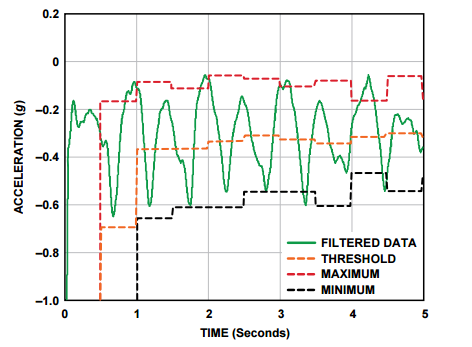
\includegraphics[scale=0.8]{Images/accPlot.png}
  \caption{A acceleration plot from \citet[p. 2]{zhao:pedometer} showing filtered data from a pedometer worn by a person walking}
  \label{fig:zhaoGraph}
\end{figure}


\subsection{Calculation of Steps Per Minute}
The gab between steps are used to calculate the number of steps the user takes per minute (SPM).

First, the amplitude is calculated which represents the change x, y, z values obtained from the accelerometer. The formula used for this is $$amplitude = \sqrt{x^{2} + y^{2} + z^{2}}$$

The array containing accelerometer measurement data is then updated with the newly calculated value. The data in this array is used for determining whether a step is taken or not, the implementation of which is described in \Cref{sec:stepCnt}.

If we detect a step we look when the previous step was taken and calculate SPM from that, this value is then stored in the array containing the SPM measurements. Afterwards, the average value of the SPM array with the new value is calculated, and the GUI is updated with a new value through a GUI manager.

If no step is taken and more than 2 seconds have passed, the implementation interprets this as if no steps are being taken and the SPM array and GUI is updated with the value 0.